\documentclass[12pt,a4paper]{book} % article, report, book.
%%%%%%%%%%%%%%%%%%%%%%%%%%%%%%%%%%%%%%%%%%%%%%%%%%%%%%%%%%%%%%%%%%%
%%% Documento LaTeX                                             %%%
%%%%%%%%%%%%%%%%%%%%%%%%%%%%%%%%%%%%%%%%%%%%%%%%%%%%%%%%%%%%%%%%%%%
% Título: Paquetes
% Autor:  Ignacio Moreno Doblas
% Fecha:  2014-02-01
%%%%%%%%%%%%%%%%%%%%%%%%%%%%%%%%%%%%%%%%%%%%%%%%%%%%%%%%%%%%%%%%%%%
% Tabla de materias:
% 1 Codificación e idioma %
% 2 Matemáticas y Física %
% 3 Gráficos%
% 4 Estilo y formato%
%%%%%%%%%%%%%%%%%%%%%%%%%%%%%%%%%%%%%%%%%%%%%%%%%%%%%%%%%%%%%%%%%%%

%1 Codificación e idioma%
\usepackage[utf8]{inputenc} %Codificación en utf8%
\usepackage[spanish]{babel} %Hyphenation (Guionado) en español%
\usepackage[T1]{fontenc} %Codificación de fuente%
\usepackage{eurofont} %Tipografía euro (€)%

%2 Matemáticas y Física %
% Importante para ecuaciones, magnitudes y unidades%
\usepackage{amssymb,amsmath,latexsym,amsfonts} % paquetes estándar%
\usepackage[squaren]{SIunits} %Paquete para magnitudes y unidades físicas%
\usepackage{ifthen} %sentencias if y while%

%3 Gráficos%
\usepackage{graphics,graphicx} %paquetes gráficos estándar%
\usepackage{wrapfig} %paquete para gráfica lateral%
\usepackage[rflt]{floatflt} %figuras flotantes%
  % \begin{floatingfigure}[r]/[l]{4.5cm}
  % \end{floatingfigure}
\usepackage{graphpap} %comando \graphpaper en el entorno picture%

%4 Estilo y formato%
\usepackage{fancyhdr} %cabeceras y pies mejor que con \pagestyle{}%
\usepackage{titlesec,titletoc} %Formateo de secciones y títulos%
\raggedbottom %Para fragmentar versos en varias páginas%
\usepackage{makeidx} %MakeIndex%
%\usepackage{showidx} % Hace que cada comando \index se imprima en la página donde se ha puesto (útil para corregir los índices)
\usepackage{alltt} % Define el environment alltt, como verbatim, excepto que \, { y } tienen su significado normal. Se describe en el fichero alltt.dtx.
\usepackage[pdftex,bookmarksnumbered,hidelinks]{hyperref} %hyper-references%
\usepackage{minitoc} % Para poner tablas de contenido en cada capítulo.
\usepackage{listings} % Para escribir piezas de código C, Python, etc. %
%listings configuration
\lstset{
  language=[ARM]Assembler, %Puede ser C, C++, Java, etc.
  showstringspaces=false,
  formfeed=\newpage,
  tabsize=4,
  commentstyle=\itshape,
  basicstyle=\ttfamily,
  morekeywords={models, lambda, forms}
}

\usepackage{tipa} % tipografía IPA (International Phonetic Alphabet)
\usepackage{longtable} %Entorno Longtable, fracciona tablas a lo largo de páginas%
\usepackage{colortbl}
\usepackage{acronym}  %Para expandir automáticamente los acrónimos

%%%%%%%%%%%%%%%%%%%%%%%%%%%%%%%%%%%%%%%%%%%%%%%%%%%%%%%%%%%%%%%%%%%
% Tabla de materias:
% 1 Información del Documento %
% 2 Comandos a nivel de texto %
% 3 Comandos a nivel de entorno %
% 4 Comandos a nivel de página y sección %
% 5 Otros comandos %
%%%%%%%%%%%%%%%%%%%%%%%%%%%%%%%%%%%%%%%%%%%%%%%%%%%%%%%%%%%%%%%%%%%

% 1 Información del Documento %
\newcommand{\pfctitlename}{Guiones de prácticas sobre la plataforma Raspberry Pi}
\newcommand{\pfcauthorname}{Antonio José Villena Godoy}
\newcommand{\pfctutorname}{Rafael Asenjo Plaza \\ Francisco Javier Corbera Peña}
\newcommand{\pfcanno}{2015}

% 2 Comandos a nivel de texto %
\newcommand{\R}{\textsuperscript{\textregistered}}  %Símbolo registrado%
\newcommand{\C}{\textsuperscript{\copyright}} %Símbolo Copyright%
\newcommand{\TM}{\texttrademark} %Símbolo Trade Mark (marca comercial)%

% 2.1 Comandos abreviatura %
\newcommand{\tit}{\textit} %Fuente cursiva (itálica)%
\newcommand{\tbf}{\textbf} %Fuente negrita%
\newcommand{\ttw}[1]{\texttt{#1}} %Fuente máquina de escribir (typewriter)%
%Combinación%
\newcommand{\textittt}[1]{\textit{\texttt{#1}}} %itálica y typewriter%
\newcommand{\textittw}{\textittt} % Otra forma de escribirlo.
\newcommand{\tittw}{\textittw} %Shortened%
\newcommand{\tbftw}[1]{\tbf{\ttw{#1}}}

%Crea una nueva línea y la indenta sin crear interlineado extra.
\newcommand{\nli}{\\ \indent} 

%Para escribir un correo electrónico%
\newcommand{\mailto}[1]{\href{mailto:#1}{#1}}

% Si vas a hacer un uso básico de \index (entradas en el índice de sólo un nivel, sin formatos especiales, etc.), define la orden
\newcommand{\miindex}[1]{#1\index{#1}}

\newcommand{\hs}{\hspace} % Abreviatura espacio horizontal
\newcommand{\vs}{\vspace} % Abreviatura espacio vertical

% Abreviaturas para los conjuntos de números más comunes.
\newcommand{\realnumbers}{\mathbb R}
\newcommand{\naturalnumbers}{\mathbb N}
\newcommand{\integernumbers}{\mathbb Z}
\newcommand{\rationalnumbers}{\mathbb Q}
\newcommand{\complexnumbers}{\mathbb R}
\newcommand{\irrationalnumbers}{\mathbb I}

% Doble barra sobre una letra (para expresar las matrices).
\newcommand{\doublebar}[1]{\bar{\bar{#1}}} 
% Ej: \vector(y) = \doublebar(A) \vector(x) (Stma. lineal de ec.)

% 3 Comandos a nivel de entorno %
\newcommand{\benu}{\begin{enu}} % Begin enumerate
\newcommand{\eenu}{\end{enu}}   % End enumeration

%Comando para escribir código Python
\newcommand{\code}[3]{
  %\hrulefill
  %\subsection*{#1}
  %\subsubsection{#1}
  \lstinputlisting{#2}
  %#1\\
  \begin{table}[h!]
    \centering
    \caption{#1}
    \label{#3}
  \end{table}
  \vspace{2em}
}

% 4 Comandos a nivel de página y sección %
%Crea página en blanco
\newcommand{\blankpage}{\clearpage{\pagestyle{empty}\cleardoublepage}}

% Versión x del comando section: sin numeración pero sí aparece en la tabla de contenidos.
\newcommand{\sectionx}[1]{
  \section*{#1}
  \addcontentsline{toc}{section}{#1}
}

% Versión y del comando section: sin numeración y NO aparece en la tabla de contenidos.
\newcommand{\sectiony}[1]{
  \section*{#1}
}

% Versión x del comando chapter: sin numeración pero sí  aparece en la tabla de contenidos.
\newcommand{\chapterx}[1]{
  \chapter*{#1}
  %\addcontentsline{toc}{chapter}{#1} %Caused by minitoc package%
  \addstarredchapter{#1} %For minitoc package%
}

% substituto del comando \chapter: incluye estilo de página.
\newcommand{\chapterbegin}[1]%
  {%
    \pagestyle{fancy}
    \fancyhead[LE,RO]{\thepage}
    \fancyhead[LO]{Capítulo \thechapter. #1}
    %\fancyhead[RE]{Parte \thepart \rightmark} %
    \fancyhead[RE]{\nouppercase{\rightmark}} %
        
    \chapter{#1}
  }

% Versión x del comando \chapterbegin: sin numeración y aparece en la tabla de contenidos.
\newcommand{\chapterbeginx}[1]%
  {%
    \pagestyle{fancy}
    \fancyhead[RO,LE]{\thepage}
    \fancyhead[RE,LO]{#1}
    %\fancyhead[LO]{Chapter \thechapter}
    %\fancyhead[RE]{Part \thepart} %
    
    \chapterx{#1}
  }

%Fin de capítulo
\newcommand{\chapterend}{\pagestyle{empty}\cleardoublepage \thispagestyle{empty}}
%Si fuera un artículo en lugar un libro, \clearpage en lugar de \cleardoublepage

% 5 Otros comandos %
%\let\Oldpart\part
%\newcommand{\parttitle}{}
%\renewcommand{part}[1]{\Oldpart{#1}\renewcommand{\parttitle}{#1}} %Header customization%

%Cambiar el título índice de capítulo a ``Contenido''.
\renewcommand{\mtctitle}{Contenido}

\dominitoc % Para tablas de contenidos por capítulo.

\addto{\captionsspanish}{
  \renewcommand{\listtablename}{Índice de Tablas}
  \renewcommand{\tablename}{Tabla} } % Por ejemplo, modificar el nombre de 'Cuadro' a 'Tabla'.

\addto{\captionsspanish}{
  \renewcommand{\contentsname}{Índice} }

%Si se desea cambiar el tipo de letra a Arial
% por cualquier razón, descomentar las siguientes
% dos líneas
%\renewcommand{\rmdefault}{phv} % Arial
%\renewcommand{\sfdefault}{phv} % Arial
  
%\addto{\captionsspanish}{
% \renewcommand{\partname}{Fase} }

%\addto{\captionsspanish}{%
%    \renewcommand{\refname}{\vspace{-4.5ex}}} % Para que no aparezca el texto 'referencias' en la bibliografía.

% Modifica el interlineado
%\renewcommand{\baselinestretch}{1.5}

   \definecolor{myfboxbg}{gray}{0.9}
   \newsavebox{\efcaja}
   \newenvironment{myfbox}{\begin{lrbox}{\efcaja}}
               {\end{lrbox}{\colorbox{myfboxbg}{\usebox{\efcaja}}}}

%%%%%%%%%%%%%%%%%%%%%%%%%%%%%%%%%%%%%%%%%%%%%%%%%%%%%%%%%%%%%%%%%%%
% Tabla de materias:
%--------------------%
% 1 dobleindent
% 2 izqindent
% 3 dobleindentx
% 4 ite
% 5 descript
% 6 enu
% 7 itemization
% 8 sinopsis
% 9 objetivo
%%%%%%%%%%%%%%%%%%%%%%%
% Para conocer los parámetros de diseño de las listas, tales como
%  los márgenes izquierdo, derechos y los diferentes saltos,
%  véase el archivo ``List layout.png'' que acompaña esta plantilla.
% Así se conocerá mejor cómo adaptar un entorno según los requisitos 
%  del usuario.

%%%%%%%%%%%%%%%%%%%%%%%
% Definición de longitudes para usar en los entornos:
%
% Normal parskip.
\newlength{\parskipenv}
\setlength{\parskipenv}{\parskip}

\newlength{\parindentenv}
\setlength{\parindentenv}{\parindent}
%%%%%%%%%%%%%%%%%%%%%%%

% 1 dobleindent
%El entorno dobleindent está pensando para escribir párrafos con doble indentación a cada lado.
%Tiene dos parámetros de entrada con las distancias medidas desde los márgenes de página.

\newenvironment{dobleindent}[2]
  %Comienzo de nuevo entorno%
  {
  \begin{list}
    {}
    {
    % Left and right margins:
    \leftmargin = #1 
    \rightmargin = #2
    %
    % Separation from preceding and following text:
    \topsep = 0ex
    \partopsep = 0ex
    \parsep = \parskipenv
    %
    % Indentation for paragraphs:
    \itemsep = \parskipenv
    \itemindent = \parindentenv
    \listparindent = \itemindent
    %
    % Horizontal separation from label:
    \labelsep = 1ex
    \settowidth{\labelwidth}{0cm}
    }
    
     \item}
  % End new env
  {\end{list}}

%%%%%%%%%%%%%%%%%%%%%%%%%%%%%
%2 izqindent
% El entorno izqindent sólo crea un párrafo indentado a la izquierda.
\newenvironment{izqindent}[1]
{
\begin{dobleindent}{#1}{0cm}
}
{
\end{dobleindent}
}

%%%%%%%%%%%%%%%%%%%%%%%%%%%%%
% 3 dobleindentx
% El entorno dobleindentx es una variación del dobleindent usando leftskip y rightskip.
% Aunque es más limitado, también se puede usar.
\newenvironment{dobleindentx}[2] % Sólo funciona en modo paragraph
{ % Preamble
  \leftskip = #1
  \rightskip = #2
}
{ % Postamble
\leftskip = 0cm
\rightskip = 0cm
}

%%%%%%%%%%%%%%%%%%%%%%%%%%%%%
% 4 ite
% El entorno ite es una modificación del entorno itemize estándar de \LaTeX. Puede usarse o modificarse si el usuario lo desea.
% También puede parametrizarse el entorno enumerate o description de forma equivalente.
\newenvironment{ite}
  {
    \begin{izqindent}{\parindent}
    \hspace{-\parindent}  % compensación del sangrado que introduce el entorno.
    \vspace{-1.0\parskip} % compensación del \parskip que introduce el entorno.
    \vspace{-\baselineskip} % compensación por la línea que introduce el entorno.
    \begin{itemize}
  }
  {
    \end{itemize}
    \end{izqindent}
  }

%%%%%%%%%%%%%%%%%%%%%5
% commando stdformat para formatear los entornos descript, enu y itemization.
\newcommand{\stdformat}
  {% Declarations for format presentation.
    %     
    % Separation from preceding and following text:
    \setlength{\topsep}{0ex}%
    \setlength{\partopsep}{0ex} %
    %
    % Horizontal separation from label:
    \labelsep = 1ex
    \setlength{\labelwidth}{0ex}
    %
    % Left and right margins: 
    \setlength{\leftmargin}{1cm}%
    \addtolength{\leftmargin}{\labelsep}
    \setlength{\rightmargin}{0ex}
    %  
    % Indentation for paragraphs:
    \setlength{\itemindent}{-\leftmargin}%
    \addtolength{\itemindent}{1ex}
    \setlength{\listparindent}{\parindent}%
    %   
    % Separation between paragraphs.
    \setlength{\parsep}{\parskipenv}% 
    \setlength{\itemsep}{1ex}
  }

%%%%%%%%%%%%%%%%%%%%%%%%%%%%%
% 5 descript

\newenvironment{descript}
  % Beginning new env def.
  {
    \begin{list}
      {} % No default label for \item.
      {
        % Declarations for format presentation.
        \stdformat
        %
        \renewcommand{\makelabel}[1]{\normalfont\bfseries##1\hfil}
      }
  }
  % Ending new env def.
  {
    \hspace*{\fill} \\ \end{list}
  } % Se introduce un salto de línea para que el texto siguiente esté separado.
%END newenvironment{descript}

%%%%%%%%%%%%%%%%%%%%%%%%%%%%%
% 6 enu
\newcounter{itemnumber} % Counter for the environment.

\newenvironment{enu}
  % Beginning new env def.
  {
    \begin{list}
    {
      \raggedleft \arabic{itemnumber}
    }
    {
      \usecounter{itemnumber}
      \stdformat
    }
  }
  {
    \end{list}
  }

%%%%%%%%%%%%%%%%%%%%%%%%%%%%%
% 7 itemization
\newenvironment{itemization}
  % Beginning new env def.
  {
    \begin{list}
      {$\bullet$} % No default label for \item.
      {
        % Declarations for format presentation.
        \stdformat
      }
  }
  % Ending new env def.
  {
    \end{list}
  }


%%%%%%%%%%%%%%%%%%%%%%%%%%%%%
% 8 sinopsis
\newenvironment{sinopsis}{%[1]{
  \sectiony{Sinopsis}
  %\label{#1}
} {
  \pagebreak
}

%%%%%%%%%%%%%%%%%%%%%%%%%%%%%
% 9 objetivo
\newenvironment{objetivo}{%[1]{
  \sectiony{Objetivo}
  %\label{#1}
} {
}

%%%%%%%%%%%%%%%%%%%%%%%%%%%%%%%%%%%%%%%%%%%%%%%%%%%%%%%%%%%%%%%%%%%
% Tabla de materias:
%--------------------%
% 1 Márgenes de página
%%%%%%%%%%%%%%%%%%%%%%%
% Para conocer los parámetros de diseño de páginas, tales como
%  los márgenes izquierdo, derecho, anchura de página, etc.
%  véase el archivo ``Page layout.png'' que acompaña esta plantilla.
% Así se conocerá mejor cómo adaptar el documento según los 
%  requisitos del usuario.

% 1 Márgenes de página
%-------------------------------%
% Parámetros de estilo de página.
% DIN A4: 29.7 cm x 21 cm
%   área neta: 3 cm + 3 cm + 15 cm.
%
% Definición de márgenes de página
%  even para páginas pares
%  odd  para páginas impares
\newlength{\realoddsidemargin}    % \oddsidemargin menos 1 in.
\newlength{\realevensidemargin}   % \evensidemargin menos 1 in.
\newlength{\realtopmargin}        % \topmargin menos 1 in.
%
% Asignación de márgenes de página
% ASIGNESE en caso de querer cambiarlo
\setlength{\realtopmargin}{2cm}     % REAL top margin.
\setlength{\realoddsidemargin}{3cm}   % REAL oddside margin.
\setlength{\realevensidemargin}{3cm}  % REAL evenside margin.
\setlength{\hoffset}{0cm}
\setlength{\voffset}{0cm}
%
% Substracción de 1 pulgada de compensación
%  (véase ``Page Layout.png'' para más información)
\addtolength{\realoddsidemargin}{-1in}  % 1 inch = 2.54 cm.
\addtolength{\realevensidemargin}{-1in}
\addtolength{\realtopmargin}{-1in}
%
% Asignación de anchuras y márgenes
% No hay notas al margen
\setlength{\marginparsep}{0cm} % No van a existir notas al margen
\setlength{\marginparwidth}{0cm} % No van a existir notas al margen
%
% Asignación de anchura de texto
\setlength{\textwidth}{15cm}  % Anchura neta del texto (globalmente).
%
% Asignación de márgenes par, impar y en altura
\setlength{\oddsidemargin}{\realoddsidemargin}  % odd-page left margin (global).
\setlength{\evensidemargin}{\realoddsidemargin} % even-page left margin (global).
\setlength{\topmargin}{\realtopmargin}          % top margin (Global).

% Se puede usar también el paquete chngpage.

%%%%%%%%%%%%%%%%%%%%%%%%%%%%%%%%%%%%%%%%%%%%%%%%%%%%%%%%%%%%%%%%%%
%   1 Length commands.          %
%-------------------------------%
% Defines new length command (e.g., \newlength{\gnat}}
% \newlength{}
%
% Set lenght to a value.
% \setlength{\gnat}{length}
% \addtolength{}{}
%
% Sets the value of a length command equal to the width of a specified piece of text; e.g., \settowidth{\parindent}{\em small}.
% \settowidth{}{}
% Set the value of a height. e.g., \settoheight{\parskip}{Gnu}
% \settoheight{}{}
% Set the value that extends below the line. e.g., \settodepth{\parskip}{gnu}.
% \settodepth{}{}
%
% To multiply a length, write: 7.0\gnat = \gnat * 7.0
%%%%%%%%%%%%%%%%%%%%%%%%%%%%%%%%%%%%%%%%%%%%%%%%%%%%%%%%%%%%%%%%%%

\begin{document}

%%%%%%%%%%%%%%%%%%%%%%%%%%%%%%%%%%%%%%%%%%%%%%%%%%%%%%%%%%%%%%

\chapterbegin{Interrupciones hardware}
\label{chp:Interrupciones}
\minitoc

{\bf Objetivos}: En esta sesión vamos a realizar programas que
utilizan dispositivos de E/S haciendo uso del sistema de
interrupciones hardware. Para poder programar los distintos parámetros
que configuran el entorno de las interrupciones es necesario conocer de
forma detallada cómo funcionan los registros asociados, ya que
éste es el mecanismo mediante el cual el procesador se
comunica con los periféricos.

Hacemos incapié en lo de {\it hardware} porque las
{\it interrupciones software} no son más que las llamadas a sistema
que vimos en el capítulo anterior. Ambas comparten vector de interrupciones,
pero las {\it interrupciones software} son más bien llamadas a subrutinas.

\section{Lectura previa}

\subsection{Hardware necesario}

Como vamos a seguir trabajando en {\it Bare Metal} y la complejidad
de los ejemplos va en aumento, no nos queda más remedio que
recurrir a hardware externo a la Raspberry para poder seguir. Se
trata de una placa sencilla, con 2 pulsadores, 6 LEDs y un altavoz
piezoeléctrico.

\begin{longtable}{ p{1.8cm} | p{1.2cm} | p{2cm} | p{5cm}}
\hline
{\bf Nombre} & {\bf GPIO} & {\bf Tipo} & {\bf Descripción} \\ \hline
LED1 & 0/2 & Salida & Diodo led color rojo \\ \hline
LED2 & 1/3 & Salida & Diodo led color rojo \\ \hline
LED3 & 17 & Salida & Diodo led color amarillo \\ \hline
LED4 & 22 & Salida & Diodo led color amarillo \\ \hline
LED5 & 10 & Salida & Diodo led color verde \\ \hline
LED6 & 11 & Salida & Diodo led color verde \\ \hline
BOT1 & 21/27 & Entrada & Pulsador izquierdo \\ \hline
BOT2 & 9 & Entrada & Pulsador derecho \\ \hline
ALT & 4 & Salida & Altavoz piezoeléctrico \\ \hline
\label{tab:berry}
\end{longtable}

Es un circuito sencillo y se puede montar en una protoboard sin
problemas, el esquema es el siguiente.

\begin{figure}[h]
  \centering
    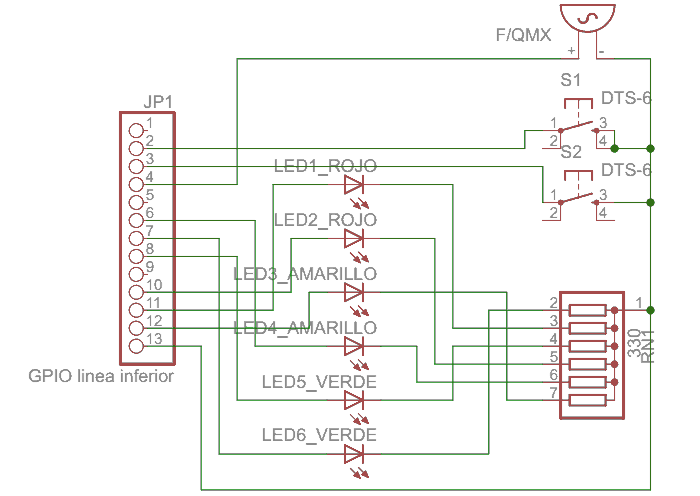
\includegraphics[width=14cm]{graphs/circuito.png}
  \caption{Esquema del circuito}
  \label{fig:circuito}
\end{figure}

También se pueden adquirir por internet tarjetas similares, aunque cableadas
a distintos puertos GPIO, por lo que habría que hacer los respectivos cambios
en el código de los ejemplos.

\subsection{Conceptos previos}

Una interrupción es una petición que se hace a la CPU para que detenga el
trabajo que esté realizando y ejecute una rutina determinada. Es uno de los
dos métodos que hay para comunicarse con los periféricos. El otro método,
que ya hemos usado en el capítulo anterior, se llama {\it Polling} y no es
más que una consulta constante sobre el estado de un periférico o un envío
continuo de información.

Existe otro concepto llamado {\it Excepción} que es muy ambiguo. Normalmente
una excepción es una situación de error detectada por la CPU mientras ejecuta
una instrucción, que requiere tratamiento por parte del sistema operativo.
Sin embargo en lo que a arquitectura ARM se refiere, el concepto {\it Excepción}
es diferente. Se trata de un caso general y abarca interrupciones hardware,
interrupciones software y el caso particular de {\it excepción} que explicamos
antes.

Por último tenemos el vector de excepciones, que no es más que una serie de
direcciones a las que la CPU saltará según el tipo de excepción que se produzca.
Lo más normal es que la base del vector de excepciones sea la dirección {\tt 0x00000000},
o sea la dirección más baja de memoria, aunque se puede cambiar dicha dirección base.
La lista del vector de excepciones es la siguiente.

\begin{longtable}{ p{5cm} | p{2cm} | p{4cm}}
\hline
{\bf Excepción} & {\bf Desplaz.} & {\bf Modo} \\ \hline
Reset                   & {\tt 0x00} & Supervisor \\ \hline
Instrucción no definida & {\tt 0x04} & No definido \\ \hline
Interrupción software   & {\tt 0x08} & Supervisor \\ \hline
Error en prefetch       & {\tt 0x0C} & Abort \\ \hline
Error en datos          & {\tt 0x10} & Abort \\ \hline
Reservado               & {\tt 0x14} & Reservado \\ \hline
IRQ                     & {\tt 0x18} & IRQ \\ \hline
FIQ                     & {\tt 0x1C} & FIQ \\ \hline
\end{longtable}

La última columna se refiere al {\it Modo de operación} que comentamos en el primer
capítulo, es un estado en el que se encuentra el procesador con una serie de privilegios
con respecto a otros modos y que gracias a ellos podemos construir un sistema operativo
con diferentes capas. Cada modo tiene sus propios registros {\tt sp} y {\tt lr} de tal
forma que no alteramos la pila de la secuencia de programa que interrumpimos. Incluso
el modo {\tt FIQ} tiene 5 registros generales propios (desde {\tt r8} hasta {\tt r12}),
de esta forma si los empleamos en nuestra rutina de tratamiento no tendremos que
salvaguardarlos en pila.

{\it Reset} es la excepción que se produce al forzar un reinicio en dicha máquina. La
Raspberry no tiene pulsador de reset, pero sí un par de pines (sin montar) para que podamos
añadir un pulsador externo. Este conector se llama {\tt P6} en la Raspberry original y
{\tt RUN} en el modelo B+.

{\it Instrucción no definida} se produce cuando en el flujo de instrucciones nos encontramos
un código de operación que no se corresponde con ninguna instrucción. Normalmente esto se
produce por una corrupción en la memoria de programa o bien que hemos saltado erróneamente
a una zona donde hay datos. También se puede dar el caso de que intentemos ejecutar código
ARM para una plataforma más moderna y nos encontremos con una instrucción no soportada por el
procesador que tenemos.

Las {\it interrupciones software} ya las hemos visto, son las que se invocan con la
instrucción {\tt swi \#n}.

Luego tenemos los errores en {\it prefetch} y {\it datos}. Un error de {\it prefetch} se produce
cuando tratamos de ejecutar una instrucción que momentos antes hemos modificado. Es poco
frecuente y para que se produzca debemos escribir código que sea automodificable, que es
una práctica no deseable y apenas utilizada en dicha arquitectura. Los errores de {\it datos}
son generados normalmente por el manejador de memoria y responden a fallos de alineación, de
traslación, de dominio o de permisos.

Lo siguiente es una entrada reservada, no tiene ninguna funcionalidad ahora
pero es probable que en futuras extensiones sí que la tenga.

Por último están las excepciones que nos interesan y que trataremos en este capítulo, que son
las interrupciones normales {\tt IRQ} y las interrupciones rápidas {\tt FIQ}.

\subsection{Rutina de tratamiento de interrupción}

Es el segmento de código que se ejecuta para atender a una interrupción. Una vez se haya
ejecutado dicha rutina, retomamos la ejecución normal de nuestro programa, justo en la instrucción en
donde lo habíamos interrumpido. Cada rutina de tratamiento debe atender a todas las posibles
fuentes de interrupción de su mismo tipo, con lo que al comienzo de la interrupción se suelen
acceder a los registros asociados para detectar qué periférico ha causado la excepción y
actuar en consecuencia.

Como sólo nos interesan {\tt IRQ} y {\tt FIQ}, a lo sumo sólo tendremos que escribir dos
rutinas de tratamiento distintas. Si se produce una {\tt IRQ}, se ejecutará el código
que se encuentre en la dirección {\tt 0x0018}, mientras que si lo que salta es una {\tt IRQ},
la dirección a ejecutar será {\tt 0x001C}. La diferencia entre una {\tt IRQ} y una
{\tt FIQ} es que esta última tiene sus propios registros desde {\tt r8} hasta {\tt r12}
asociados al modo de operación, con lo que podemos prescindir del salvado y recuperación
de estos registros en la RTI, ahorrando un tiempo que en determinadas aplicaciones de
tiempo real puede ser decisivo.

El esqueleto de una RTI es el siguiente.

\begin{lstlisting}
irq_handler:
        push    {lista registros}
        ...
        pop     {lista registros}
        subs    pc, lr, #4
\end{lstlisting}

Vemos que a diferencia de las subrutinas donde salíamos con {\tt lr}, en una RTI salimos
con {\tt lr-4}, a ello se debe la última instrucción. ¿Y porqué hay un sufijo {\tt s} al final
de la instrucción {\tt sub}? Pues porque se trata de instrucción especial que sirve para
restaurar el registro {\tt cpsr} que había antes de la interrupción.

Cada modo de operación tiene 3 registros replicados: {\tt sp}, {\tt lr} y {\tt spsr}. Cuando
ocurre una interrupción pasamos de modo supervisor a modo IRQ. Los registros {\tt sp}
y {\tt lr} del modo supervisor no se tocan para nada, con lo que tenemos nuestra propia pila
de interrupciones IRQ. El registro {\tt lr} (asociado a IRQ) se carga apuntando a la
instrucción que va después de donde se ha producido la excepción. Además se hace una copia
del registro {\tt cpsr} a otro llamado {\tt spsr} (Saved Program Status Register), porque
dentro de la RTI es probable que queramos modificar {\tt cpsr} y también porque el hecho
de cambiar de modo de operación a IRQ ya ha modificado el registro {\tt cpsr}.

Al terminar la interrupción restauramos {\tt pc} partiendo {\tt lr} y {\tt cpsr} del registro
{\tt spsr}. Al cambiar de modo volvemos al {\tt sp} y {\tt lr} que teníamos en dicho modo,
el resto de registros es responsabilidad nuestra devolverlos al valor que tenían al entrar
en la RTI. Con todo esto conseguimos volver exactamente al punto del que partíamos minimizando las
operaciones que tiene que hacer la RTI y por tanto el retardo asociado. En otras arquitecturas
además de delegar en la RTI este trabajo, se usa la misma pila de programa, lo que puede
ocasionar problemas si nos importa lo que hay debajo de ésta.

\subsection{Inicialización en programa principal}

En realidad la inicialización es lo único que vamos a tener en nuestro programa principal,
puesto que una vez configuradas las interrupciones vamos a controlar el comportamiento del
programa con las mismas. Es decir, nuestro programa principal tras la inicialización será una
instrucción que salta a sí misma continuamente, la misma {\tt infi: b infi} del capítulo
anterior salvo que esta vez no la usamos para dejar al sistema colgado.

El orden recomendado es el siguiente, aunque se pueden cambiar el mismo salvo el último punto.

\begin{itemize}
  \item Escribimos en el vector de excepciones de la dirección de comienzo de la RTI que vayamos
        a usar. En nuestros ejemplos tendremos IRQs y FIQs, por lo que como mucho haremos dos
        escrituras (para dos RTIs distintas).
  \item Inicializamos el puntero de pila (registro {\tt sp}) en todos los modos de operación.
        Tienen que apuntar a zonas distintas dondo sepamos que no habrá conflictos con la
        memoria de programa. En todos los ejemplos que veremos inicializamos la pila de FIQ
        a {\tt 0x4000}, la de IRQ a {\tt 0x8000} y la del modo Supervisor a {\tt 0x8000000}.
  \item Escribimos código de inicialización ajeno al proceso de interrupción, como por ejemplo
        configurar los GPIOs a salidas donde queramos que actúe un LED.
  \item Ahora viene la inicialización de las interrupciones. Aquí le decimos al sistema qué fuentes
        pueden provocar interrupciones, escribiendo en los registros asociados. 
  \item El último paso es habilitar las interrupciones globalmente escribiendo en el registro
        {\tt cpsr}. Lo hacemos indirectamente vía otro registro, y la instrucción tiene otro
        nombre pero hace lo mismo que un {\tt mov}. En concreto se llama {\tt msr}, y también hay
        otra equivalente {\tt mrs} si lo que queremos es leer de {\tt cpsr} a un registro.
  \item Después de esto se acaba la inicialización y tendríamos el bucle infinito del que consta
        nuestro programa principal. Si todo ha ido bien las rutinas de tratamiento de interrupción
        se encargarán de hacer funcionar nuestro programa como queramos.
\end{itemize}

Existen mucha formas de escribir en el vector de excepciones. Se puede rellenar toda la tabla
y hacer un copiado, o ir escribiendo uno a uno los vectores. También hay varias formas de hacer
los saltos dentro de la tabla, mediante un salto sencillo que está limitado a +/- 32Mb, o usando
la instrucción {\tt ldr pc, =valor}. Esta última requiere 4 bytes adicionales, pero a su favor
tiene que no hay limitaciones en el salto y que podemos escribir directamente la dirección
absuluta de nuestra RTI.

Nosotros vamos a emplear una función que recibe dos parámetros (dirección de vector y dirección de
RTI) y que se encargará él mismo de introducir una instrucción de salto en el lugar adecuado.

\begin{lstlisting}
add_exception:
        sub     r1, r0
        lsr     r1, #2
        sub     r1, #2
        orr     r1, #0xea000000
        str     r1, [r0]
        bx      lr
\end{lstlisting}

Habría que hacer tantas llamadas a esta función como tipos de excepciones tengamos. Luego tenemos
que inicializar los punteros de pila de los distintos modos de operación. Desde el punto de vista
del ensamblador todos los registros se llaman igual, no podemos acceder a ellos por los sufijos.
Queremos inicializar {\tt r13\_svc (sp\_svc)}, {\tt r13\_fiq (sp\_fiq)} y {\tt r13\_svc (sp\_fiq)}, y
de estos dos últimos sólo el que vayamos a emplear en nuestro programa. En la figura 
\ref{fig:tablareg} tenemos los distintos registros.

\begin{figure}[h]
  \centering
    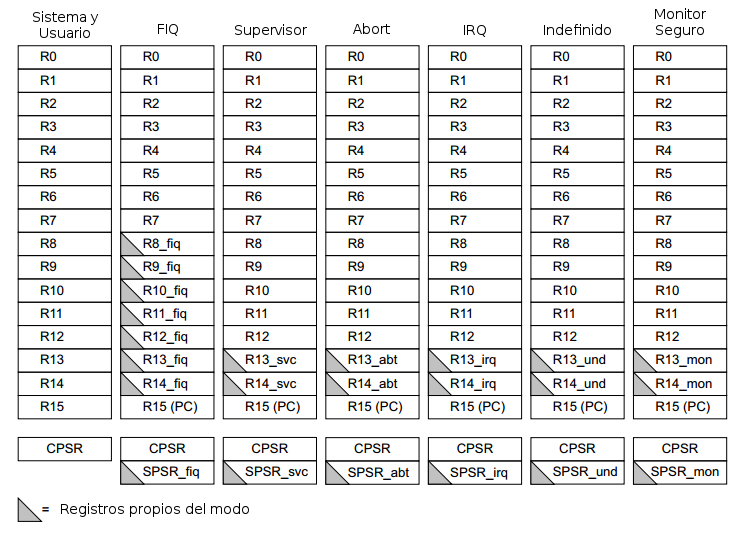
\includegraphics[width=14cm]{graphs/tablaregistros.png}
  \caption{Registros según modo de operación}
  \label{fig:tablareg}
\end{figure}

La única forma de acceder a ellos es cambiando de modo y modificando el registro {\tt sp}. En
modo {\tt Bare Metal} nos olvidamos del modo Usuario, el sistema arranca en modo Supervisor y
nosotros nos mantenemos en dicho modo a no ser que haya una interrupción, o querramos cambiar
un registro particular del modo como es el caso.

El modo viene indicado en la parte más baja del registro {\tt cpsr}, el cual modificaremos
con la instrucción especial {\tt msr}. Como sólo nos interesa cambiar el byte más bajo del
registro, añadimos el sufijo {\tt c} precedido de un guión bajo. Los otros 3 bytes se acceden
con {\tt x}, {\tt s} y {\tt f} respectivamente. En la figura \ref{fig:cpsr} vemos el contenido
completo del registro {\tt cpsr}.

\begin{figure}[h]
  \centering
    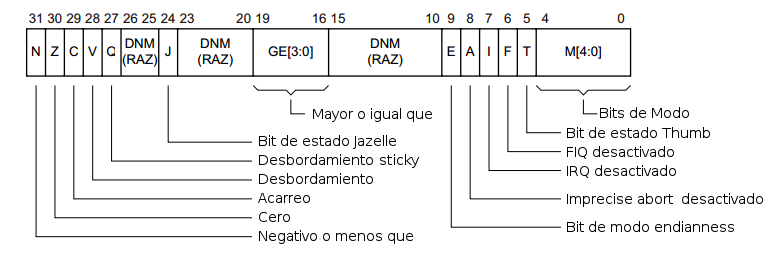
\includegraphics[width=14cm]{graphs/cpsr.png}
  \caption{Registro cpsr}
  \label{fig:cpsr}
\end{figure}

Y en la siguiente tabla vemos cómo se codifica el modo de operación.

\begin{longtable}{ p{1.8cm} | p{2cm} | p{5cm} | p{1cm} | p{1cm} }
\hline
{\bf Hex} & {\bf Binario} & {\bf Modo de operación} \\ \hline
0x10 & 10000 & Usuario        \\ \hline
0x11 & 10001 & FIQ            \\ \hline
0x12 & 10010 & IRQ            \\ \hline
0x13 & 10011 & Supervisor     \\ \hline
0x16 & 10110 & Monitor seguro \\ \hline
0x17 & 10111 & Abort          \\ \hline
0x1B & 11011 & Indefinido     \\ \hline
0x1F & 11111 & Sistema        \\ \hline
\end{longtable}

Finalmente tenemos que el código que inicializa los punteros de pila es el siguiente.

\begin{lstlisting}
        mov     r0, #0xd1     @FIQ mode, FIQ&IRQ disable
        msr     cpsr_c, r0
        mov     sp, #0x4000
        mov     r0, #0xd2     @IRQ mode, FIQ&IRQ disable
        msr     cpsr_c, r0
        mov     sp, #0x8000
        mov     r0, #0xd3     @SVC mode, FIQ&IRQ disable
        msr     cpsr_c, r0
        mov     sp, #0x8000000
\end{lstlisting}

En concreto a {\tt 0x4000}, {\tt 0x8000} y {\tt 0x8000000} para los modos {\tt FIQ}, {\tt IRQ} y
{\tt Supervisor} respectivamente.

La inicialización de las interrupciones es bastante específica, por lo que la veremos en los
respectivos ejemplos. Y por último tenemos que habilitar las interrupciones globalmente, poniendo
a cero el bit correspondiente en {\tt cpsr}, y que en el caso de habilitar IRQs sería así.

\begin{lstlisting}
        mov     r0, #0x53     @SVC mode, IRQ enable
        msr     cpsr_c, r0
\end{lstlisting}

\subsection{Ejemplos de aplicación}

Todos los ejemplos que vamos a listar son para la placa que usaremos en el laboratorio
y para los siguientes modelos de Raspberry.

\begin{itemize}
  \item Modelo A.
  \item Modelo B revisión 2.0.
  \item Modelo B+ (empleando la parte izquierda del conector).
\end{itemize}

El modelo B revisión 1.0 tiene una asignación de pines ligeramente distinta, cambiando 3 de
los pines. Si dispones de esta versión tendrías que modificar el código de los ejemplos
según la tabla \ref{tab:berry}.

\subsection{Parpadeo de todos los LEDs}

Sería hacer lo mismo que en la lección anterior pero empleando interrupciones y aplicando
la salida simultáneamente a los 6 LEDs de la placa externa en lugar del LED que incluye
la Raspberry. La cadencia debe ser de un segundo.

Vamos a emplear otro temporizador, el {\tt System Timer}, distinto al de la lección anterior
que era el {\tt ARM Timer}. Los registros asociados al temporizador son los de la figura
\ref{fig:systim}.

\begin{figure}[h]
  \centering
    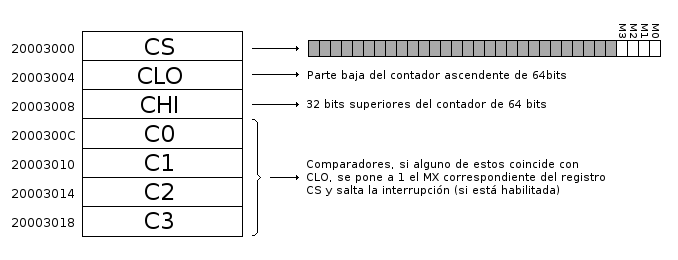
\includegraphics[width=14cm]{graphs/systemtimer.png}
  \caption{System Timer}
  \label{fig:systim}
\end{figure}

Básicamente con un contador de 64 bits y cuatro comparadores. El temporizador funciona a 1MHz,
por lo que cada microsegundo se incrementa la cuenta del contador. Está dividido en dos partes,
la parte baja {\tt CLO} y la parte alta {\tt CHI}. La parte alta no nos resulta interesante,
porque tarda poco más de una hora en incrementarse y no va asociado a ningún comparador. Los
comparadores son registros que se pueden modificar y se comparan con {\tt CLO}, en el momento
que uno de los 4 comparadores coincida y estén habilitadas las interrupciones para dicho
comparador, se produce una interrupción y se activa el correspondiente {\tt Mx}
asociado a {\tt CS} (para que en la RTI sepamos qué comparador ha provocado la interrupción).
En nuestro ejemplo vamos a usar el primer comparador o {\tt C0}.

El temporizador ya está, luego tenemos los registros asociados a las interrupciones en la figura
\ref{fig:interrupciones}.

\begin{figure}[h]
  \centering
    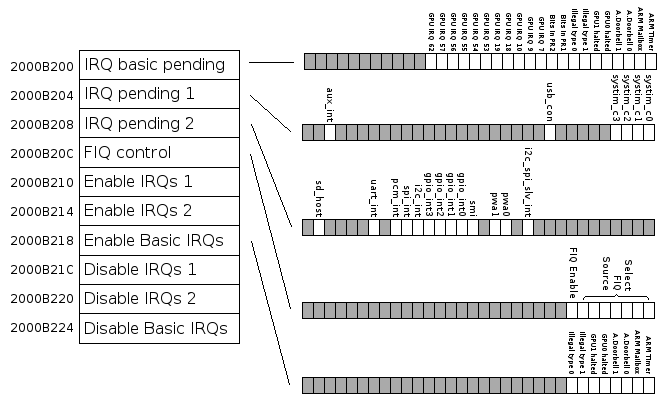
\includegraphics[width=14cm]{graphs/interrupciones.png}
  \caption{Interrupciones}
  \label{fig:interrupciones}
\end{figure}

En este caso las {\tt FIQs} sólo tienen un registro de control asociado, quedando todo el detalle
en las {\tt IRQs}. Nosotros vamos a usar las {\tt IRQs} en este ejemplo. Hay tres grupos de tres
registros cada uno. El primer grupo sirve para indicar que hay una interrupción pendiente, el
segundo es para habilitar las interrupciones y el tercero para deshabilitarlas. Dentro de cada
grupo tenemos un registro básico que tiene una mezcla de todo y otros dos registros que
indican con más detalle la fuente de la interrupción. Dentro de la mezcla del registro básico
hay fuentes individuales {\tt GPU IRQ x} y bits que engloban a varias fuentes {\tt Bits in PR1},
que por ejemplo indica que el origen hay que buscarlo en el registro 1. En el registro 1 están
las primeras 32 posiciones de la tabla de interrupciones, mientras que en el registro 2 están
las 32 últimas.

La documentación oficial sobre la tabla de interrupciones está incompleta, pero buscando un poco
por internet se puede encontrar que las interrupciones asociadas al {\tt System Timer} se
controlan con los 4 primeros bits de la tabla (uno para cada comparador).

Ya estamos en condiciones para mostrar el código del ejemplo.

\begin{lstlisting}[caption={inter1.c},label={lst:codigoPract5_1},escapeinside={@}{@}]
        .set    GPBASE,   0x20200000
        .set    GPFSEL0,        0x00
        .set    GPFSEL1,        0x04
        .set    GPFSEL2,        0x08
        .set    GPSET0,         0x1c
        .set    GPCLR0,         0x28
        .set    STBASE,   0x20003000
        .set    STCLO,          0x04
        .set    STC0,           0x0c
        .set    INTBASE,  0x2000b000
        .set    INTENIRQ1,     0x210
.text
        mov     r0, #0x18     @IRQ vector
        ldr     r1, =irq_handler
        bl      add_exception
        mov     r0, #0xd2     @IRQ mode, FIQ&IRQ disable
        msr     cpsr_c, r0
        mov     sp, #0x8000
        mov     r0, #0xd3     @SVC mode, FIQ&IRQ disable
        msr     cpsr_c, r0
        mov     sp, #0x8000000
        ldr     r0, =GPBASE
        ldr     r1, =0b00000000000000000000001001000000
        str     r1, [r0, #GPFSEL0]
        ldr     r1, =0b00000000001000000000000000001001
        str     r1, [r0, #GPFSEL1]
        mov     r1, #0b00000000000000000000000001000000
        str     r1, [r0, #GPFSEL2]
        ldr     r0, =INTBASE
        mov     r1, #1
        str     r1, [r0, #INTENIRQ1]
        mov     r0, #0x53     @SVC mode, IRQ enable
        msr     cpsr_c, r0
bucle:  b       bucle

add_exception:
        sub     r1, r0
        lsr     r1, #2
        sub     r1, #2
        orr     r1, #0xea000000
        str     r1, [r0]
        bx      lr

irq_handler:
        push    {r0, r1, r2}
        ldr     r0, =ledst
        ldr     r1, [r0]
        eors    r1, #1
        str     r1, [r0]
        ldr     r0, =GPBASE
        ldr     r1, =0b00000000010000100000110000001100
        streq   r1, [r0, #GPSET0]
        strne   r1, [r0, #GPCLR0]
        ldr     r0, =STBASE
        ldr     r1, [r0, #STCLO]
        ldr     r2, =500000
        add     r1, r2
        str     r1, [r0, #STC0]
        pop     {r0, r1, r2}
        subs    pc, lr, #4

ledst:  .word   0
\end{lstlisting}

Y vamos enumerando, por orden, los pasos que hemos seguido. En primer lugar apuntamos a nuestra
RTI en el vector de excepciones.

\begin{lstlisting}
        mov     r0, #0x18     @IRQ vector
        ldr     r1, =irq_handler
        bl      add_exception
\end{lstlisting}

Luego inicializamos los punteros de pila.

\begin{lstlisting}
        mov     r0, #0xd2     @IRQ mode, FIQ&IRQ disable
        msr     cpsr_c, r0
        mov     sp, #0x8000
        mov     r0, #0xd3     @SVC mode, FIQ&IRQ disable
        msr     cpsr_c, r0
        mov     sp, #0x8000000
\end{lstlisting}

Lo siguiente es configurar los pines GPIO asociados a los 6 LEDs como salidas.

\begin{lstlisting}
        ldr     r0, =GPBASE
        mov     r1, #0b00000000000000000000001001000000
        str     r1, [r0, #GPFSEL0]
        ldr     r1, =0b00000000001000000000000000001001
        str     r1, [r0, #GPFSEL1]
        mov     r1, #0b00000000000000000000000001000000
        str     r1, [r0, #GPFSEL2]
\end{lstlisting}

Para después habilitar las interrupciones asociadas al primer comparador {\tt C0}.

\begin{lstlisting}
        ldr     r0, =INTBASE
        mov     r1, #1
        str     r1, [r0, #INTENIRQ1]
\end{lstlisting}

Y finalmente habilitar las interrupciones {\tt IRQ} globalmente, entrando luego en
el bucle infinito.

\begin{lstlisting}
        mov     r0, #0x53     @SVC mode, IRQ enable
        msr     cpsr_c, r0
bucle:  b       bucle
\end{lstlisting}

Ya hemos terminado con el programa principal, que como veremos más adelante va a ser
siempre muy parecido.

Lo interesante está en la RTI, que es donde hacemos parpadear los LEDs y configuramos
el comparador para la siguiente interrupción.

El estado de los LEDs (si están apagados o encendidos) lo guardamos en la variable
{\tt ledst}, que conmutamos entre cero y uno mediante un {\tt OR} exclusivo. Al
actualizar los {\tt flags} tras esta operación, tenemos que si el resultado fue
cero nos lo indica el {\tt flag Z} activo, mientras que estará inactivo en el
caso contrario (resultado 1). Mediante las instrucciones de ejecución condicional
{\tt streq} y {\tt strne} enviamos la orden al puerto que enciende los LEDs o al
puerto que los apaga, respectivamente.

\begin{lstlisting}
irq_handler:
        push    {r0, r1, r2}
        ldr     r0, =ledst
        ldr     r1, [r0]
        eors    r1, #1
        str     r1, [r0]
        ldr     r0, =GPBASE
        ldr     r1, =0b00000000010000100000110000001100
        streq   r1, [r0, #GPSET0]
        strne   r1, [r0, #GPCLR0]
\end{lstlisting}

Luego tenemos que actualizar el registro comparador, de lo contrario tardará poco más
de una hora en cambiar de estado el LED (es lo que tarda el contador en dar una vuelta
completa). Para ello leemos el contador ({\tt CLO}) y le añadimos 500000 al valor leído. Como cada
cuenta equivale a un microsegundo, este añadido al contador supone medio segundo, lo
que nos da la cadencia de un segundo que buscamos. El resultado de la suma lo escribimos
en el comparador ({\tt C0}), restauramos los registros utilizados y salimos de la RTI. 

Por último tenemos la definición de la variable {\tt ledst}, como no tenemos sección de datos
aparte la ponemos al final del código.

\begin{lstlisting}
        ldr     r0, =STBASE
        ldr     r1, [r0, #STCLO]
        ldr     r2, =500000
        add     r1, r2
        str     r1, [r0, #STC0]
        pop     {r0, r1, r2}
        subs    pc, lr, #4

ledst:  .word   0
\end{lstlisting}

\subsection{Parpadeo secuencial de LEDs con sonido por altavoz}


\chapterend{}

%%%%%%%%%%%%%%%%%%%%%%%%%%%%%%%%%%%%%%%%%%%%%%%%%%%%%%%%%%%%%%
\end{document}